\section{Approximation Algorithms}
\label{sec:approx}

Because all four placement problems are NPC, we propose greedy approximation algorithms for each problem, which iteratively add 
a PMU in each step to the node that observes the maximum number of new nodes. We present two such algorithms, one that directly addresses \maxinc ({\tt greedy}) and the other 
\xvalpart ({\tt xvgreedy}). {\tt greedy} and {\tt xvgreedy} can easily be used to solve \full and \xvals, respectively, by selecting the appropriate $k$ value to ensure full observability.

{\bf {\tt greedy} Algorithm}. We start with $\Phi = \emptyset$.  At each iteration, we add a PMU to the node that results in the observation of the maximum number of 
new nodes. The algorithm terminates when all PMUs are placed.  {\footnote {\small The same greedy algorithm is proposed by Aazami and Stilp \cite{Aazami07}. }}


{\bf {\tt xvgreedy} Algorithm}. {\tt xvgreedy} is almost identical to {\tt greedy}, except that PMUs are added in pairs such that the selected pair observe
the maximum number of nodes under the condition that the PMU pair satisfy one of the cross-validation rules. % and observe the maximum number of new nodes.
%We provide the pseudo code for {\tt xvgreedy} and prove that {\tt xvgreedy} has polynomial running time in our Technical Report \cite{Tech12}. 

%Our Technical Report \cite{Tech12} gives the pseudo code for {\tt greedy} and {\tt xvgreedy} and includes proofs
%that these algorithms have polynomial complexity, making them feasible tools for approximating optimal PMU placement. 

\xxn{Aazami and Stilp prove {\tt greedy} has a $\Theta(n)$ approximation ratio under the assumption that all nodes are zero-injection.}



\subsection{The Observability Rules are Not Submodular Function}

Intuitively, submodular functions are set functions with diminishing marginal returns: the value that a single element makes in the function when added to the input set decreases
as the size of the input set increases. More formally, let $X$ be a ground set such that $|X|=n$. We define a set function on $X$ as $f: 2^X \rightarrow \mathbb{R}$.
We define a function as submodular using the definition from \footnote{\url{http://theory.stanford.edu/~shaddin/papers/submodular\_survey.pdf}}.
A set function is $f: 2^X \rightarrow \mathbb{R}$ is \emph{submodular} if, for all $A,B \subseteq X$ with $A \subseteq B$, and for each $j \in X$,
\begin{eqnarray}
f(A \cup \{j\}) - f(A) &\geq& f(B \cup \{j\}) - f(B)
\end{eqnarray}

For the PMU placement problems, we define $f(X)$ on graph, $G=(V,E)$, as the number of nodes observed by placing a PMU at each $x \in X$.  Using the example graph from
Figure \ref{fig:submodular-counter}}, we show $f$ is not submodular.  Let $A=\{a\}$ and $B=\{a,b\}$. Then,
%In this example we let $A=\{a\}$ and $B=\{a,b\}$. Then, %We show $f$ is not a submodular function
\begin{eqnarray*}
f(A \cup \{c\}) - f(A) &\stackrel{?}{\geq}& f(B \cup \{c\}) - f(B) \\
f(A \cup \{c\}) - 2 &\stackrel{?}{\geq}& f(B \cup \{c\}) - 3 \\
3-2 &\stackrel{?}{\geq}& 8 - 3 \\
1 &\stackrel{?}{\geq}& 5
\end{eqnarray*}
As a result, we conclude that $f$ is not submodular and therefore that our observability rules are not submodular functions.

Note that in this example, O2 prevented us from meeting the criteria for submodular functions.  For PMU placement $B \cup \{c\}$, we are able to apply O2 at $e$, resulting in the observation of the
chain of nodes at the top of the graph.  However, we were unable to apply O2 for PMU placement $A \cup \{c\}$.
  
%It follows that $f(A)=2$ and $f(B)=3$. 

\begin{figure}[t]
\centering
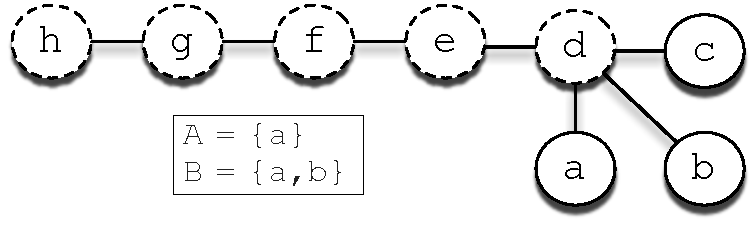
\includegraphics[scale=.75]{figs/submodular-counterexample.pdf}
\caption{Example showing the observability rules are not submodular functions.}
\label{fig:submodular-counter}
\end{figure}

\xxn{Maybe we can show it is a submodular function for certain distributions of zero-injection nodes.}


%\subsection{Example Showing Greedy is not a Submodular Function}
%
%Submodular definition from \footnote{\url{http://theory.stanford.edu/~jvondrak/CS369P-files/lec16.pdf}}.  Denote $f_A(i) = f(A+i) - f(A)$ the marginal value of $i$ with respect
%to $A$.  $f$ is submodular if for all $A \subseteq B \subseteq N$ and $i \in N \setminus B$, 
%$$ f_A(i) \geq f_B(i) $$
%
%
%Execution of {\tt greedy} using Figure \ref{fig:submodular-counter}:
%\begin{enumerate}
%	\item Add PMU to $d$.  As a result, $5$ nodes, $\{a,b,c,d,h\}$, are observed by applying O1 at $d$,  O2 cannot be applied.
%	
%	\item Add PMU to $f$.  As a result, $6$ nodes become observed $\{e,f,g,i,j,k\}$ by applying O1 at $f$ and then repeatedly applying O2 (first at $h$, then at $j$, and finally at $k$)
%
%\end{enumerate}
%
%
%\begin{figure*}[t]
%  \begin{center}
%    \subfigure[The original graph (without any PMUs).]{\label{fig:submodular-counter-step0}
%		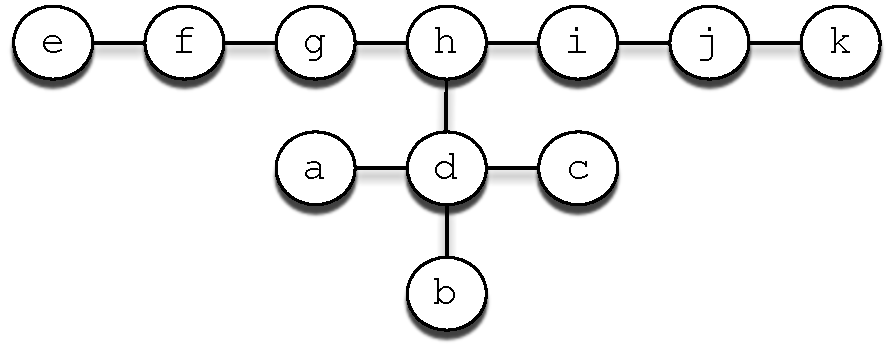
\includegraphics[scale=0.59]{figs/submodular-counterexample-step0.pdf}}
%    \subfigure[Step 1: Placing a PMU at $d$ results in the observation of $5$ nodes, $\{a,b,c,d,h\}$.]{\label{fig:submodular-counter-step1}
%		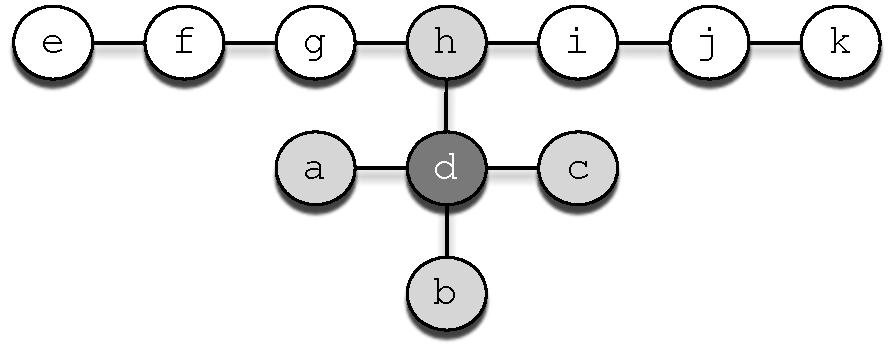
\includegraphics[scale=0.59]{figs/submodular-counterexample-step1.pdf}}
%    \subfigure[Step 2: Placing a PMU at $f$ results in the observation of $6$ nodes, $\{e,f,g,i,j,k\}$.]{\label{fig:submodular-counter-step2}
%		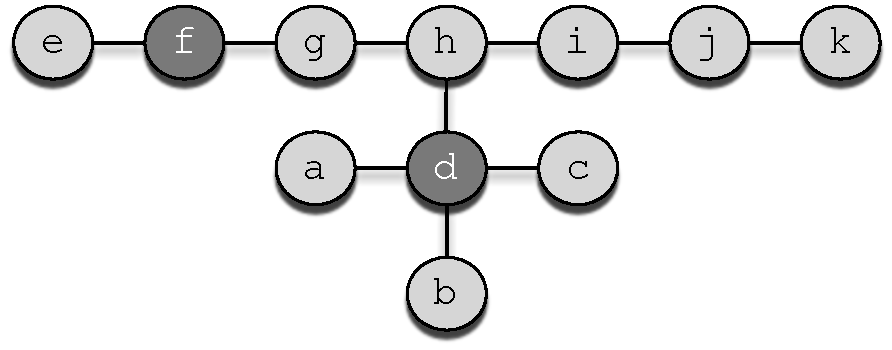
\includegraphics[scale=0.59]{figs/submodular-counterexample-step2.pdf}}
%  \end{center}
%	\caption{Example showing that {\tt greedy} is not a submodular function.} 
%	\label{fig:submodular-counter-old}
%\end{figure*}
%
%\end{comment}


%List of references explaining submodular functions.
%\footnote{Nice definition and examples. \url{http://theory.stanford.edu/~jvondrak/CS369P-files/lec16.pdf}}
%\footnote{Survey paper. \url{http://theory.stanford.edu/~shaddin/papers/submodular_survey.pdf}}
%\footnote{\url{http://en.wikipedia.org/wiki/Submodular_set_function}}
%\footnote{One of the earlier papers on submodular functions. \url{http://www.cs.toronto.edu/~eidan/papers/submod-max.pdf}}


